\chapter{\acrlong{moo}}

%%%%%%%%%%%%%%%%%   SECTION : INTRODUCTION   %%%%%%%%%%%%%%%%%%%%%%%%%%%%%%
\section{Introduction} \label{what is moo}
In today's increasingly complex world, decision-makers often face the challenge of optimizing several conflicting objectives simultaneously. \acrfull{moo} 
is an optimization that deals with such problems, where multiple objective functions are optimized simultaneously. To understand \acrshort{moo} better, 
let us consider an example.

\paragraph{Example:}
Let us consider an example of a car manufacturer. The car consists of many components like engine, body, wheels, etc which can be
tweaked. In our case, the manufacturer wants to optimize the car for two objectives: lower manufacturing cost of the car and lower carbon emissions. With 
considering the input parameters and the objectives, we get many solutions as shown in Figure \ref{moo}

\begin{figure}[!h]
	\begin{center}
		\input{../Python/plots/moo_plot.tex}
	\end{center}
    \caption{Example of \acrshort{moo}}
    \label{moo}
\end{figure}
In a \acrshort{moo} problem, there typically is no single best solution. Rather, the \textit{goal} is to identify a set of solutions that are optimal in terms 
of all objectives. In Figure \ref{moo}, the best solutions for the given objectives is indicated in orange known as pareto optimal solutions. A solution is said 
to be pareto optimal if no other solution can improve on any of the objectives without worsening at least one of the other objectives.
%The solutions which are not Pareto optimal are not considered as they are dominated by the Pareto optimal solutions. 

\section{Difference between \acrshort{moo} and \acrshort{soo}}
Optimization problems, whether single-objective or multi-objective, have the same goal: to find the best solution(s) to a given problem. However, the approach
to solving these problems is different. 

In \acrfull{soo}, the goal is to optimize a single objective function, which can either be maximized or minimized. The  problem is simpler to define and solve
because it involves only one objective. To calculate \acrshort{soo}, we can use methods like gradient descent, linear programming, etc.

\begin{figure}[!h]
    \centering
    \input{../Python/plots/soo_plot.tex}
    \caption{Example of \acrshort{soo}}
    \label{soo}
\end{figure}

In Figure \ref{soo}, we have considered the same example given in section \ref{what is moo}. But, here, we are considering only one objective, which is to
minimize the manufacturing cost. The best solution is indicated in orange.
\vspace{15pt}

In \acrshort{moo}, the optimization involves two or more objective functions simultaneously. The problem is more complex because the objectives are often
conflicting. Unlike \acrshort{soo}, where we have a single best solution, in \acrshort{moo}, we have pareto optimal solutions.
To calculate \acrshort{moo}, we can use methods like pareto optimization, scalarization method, weighted sum method, $\epsilon$-constraint method, etc.


While \acrshort{soo} focuses on finding the best solution according to a single criterion, \acrshort{moo} addresses the more complex task of balancing multiple, 
often conflicting objectives. The choice between \acrshort{soo} and \acrshort{moo} depends on the nature of the problem at hand and the goals of the decision-maker. 
Understanding the differences between these approaches is crucial for selecting the appropriate optimization technique and achieving the desired outcomes.

%#! Explain where we are currently using the MOO approach in our department

%%%%%%%%%%%%%%%   SECTION : OPTISLANG  %%%%%%%%%%%%%%%%%%%%%%%%%%%%%%%%
\section{Optislang}
\paragraph{}

To calculate \acrshort{moo}, we need a software platform that can handle the complexity of the problem. Ansys Optislang \cite{optislang} is such a software 
platform, which is used for design exploration, \acrshort{cae} based sensitivity analysis and optimization in conjunction with any product development tool. 
It is a Process Integration and Design Optimization tool or in short, a \acrshort{pido} tool. Process Integration refers to automate and orchestrate manual 
simulation processes and to realize complex workflows. Design Optimization aims for better understanding of your design, optimizing the product, identify an 
improved design which has the desired qualities and resulting in a best design by reliability analysis and statistical analysis.  


Optislang uses several solvers to look into aspects like mechanical, technical, mathematical and any other problems. This is easier in Optislang as it provides
integration to create toolchains of many external programs like ANSYS, MATLAB, Excel, Python, CATIA and many more.


Our department utilizes Optislang for solving \acrshort{moo} problems, as it includes algorithms specifically designed for \acrshort{moo}.
%# Try to explain about the parametric system, sensitivity analysis, MOP, ...
%%%%%%%%%%%%%%%%%   SECTION : MODULES AND WORKFLOWS   %%%%%%%%%%%%%%%%%%%%%%%%%%%%%%
\section{Modules and Workflows}
\subsection{Modules}
Modules are created by the system developers. Modules include a simulation model as a calculation with defined interfaces for coupling with other modules. 
These modules are either defined in MATLAB or Python. Each module is designed to tackle/improve a specific issue. To document and collaborate with other
system developers, each module is versioned and stored in a specific manner in a repository in GitHub Enterprise.

\begin{figure}[!h]
    \centering
    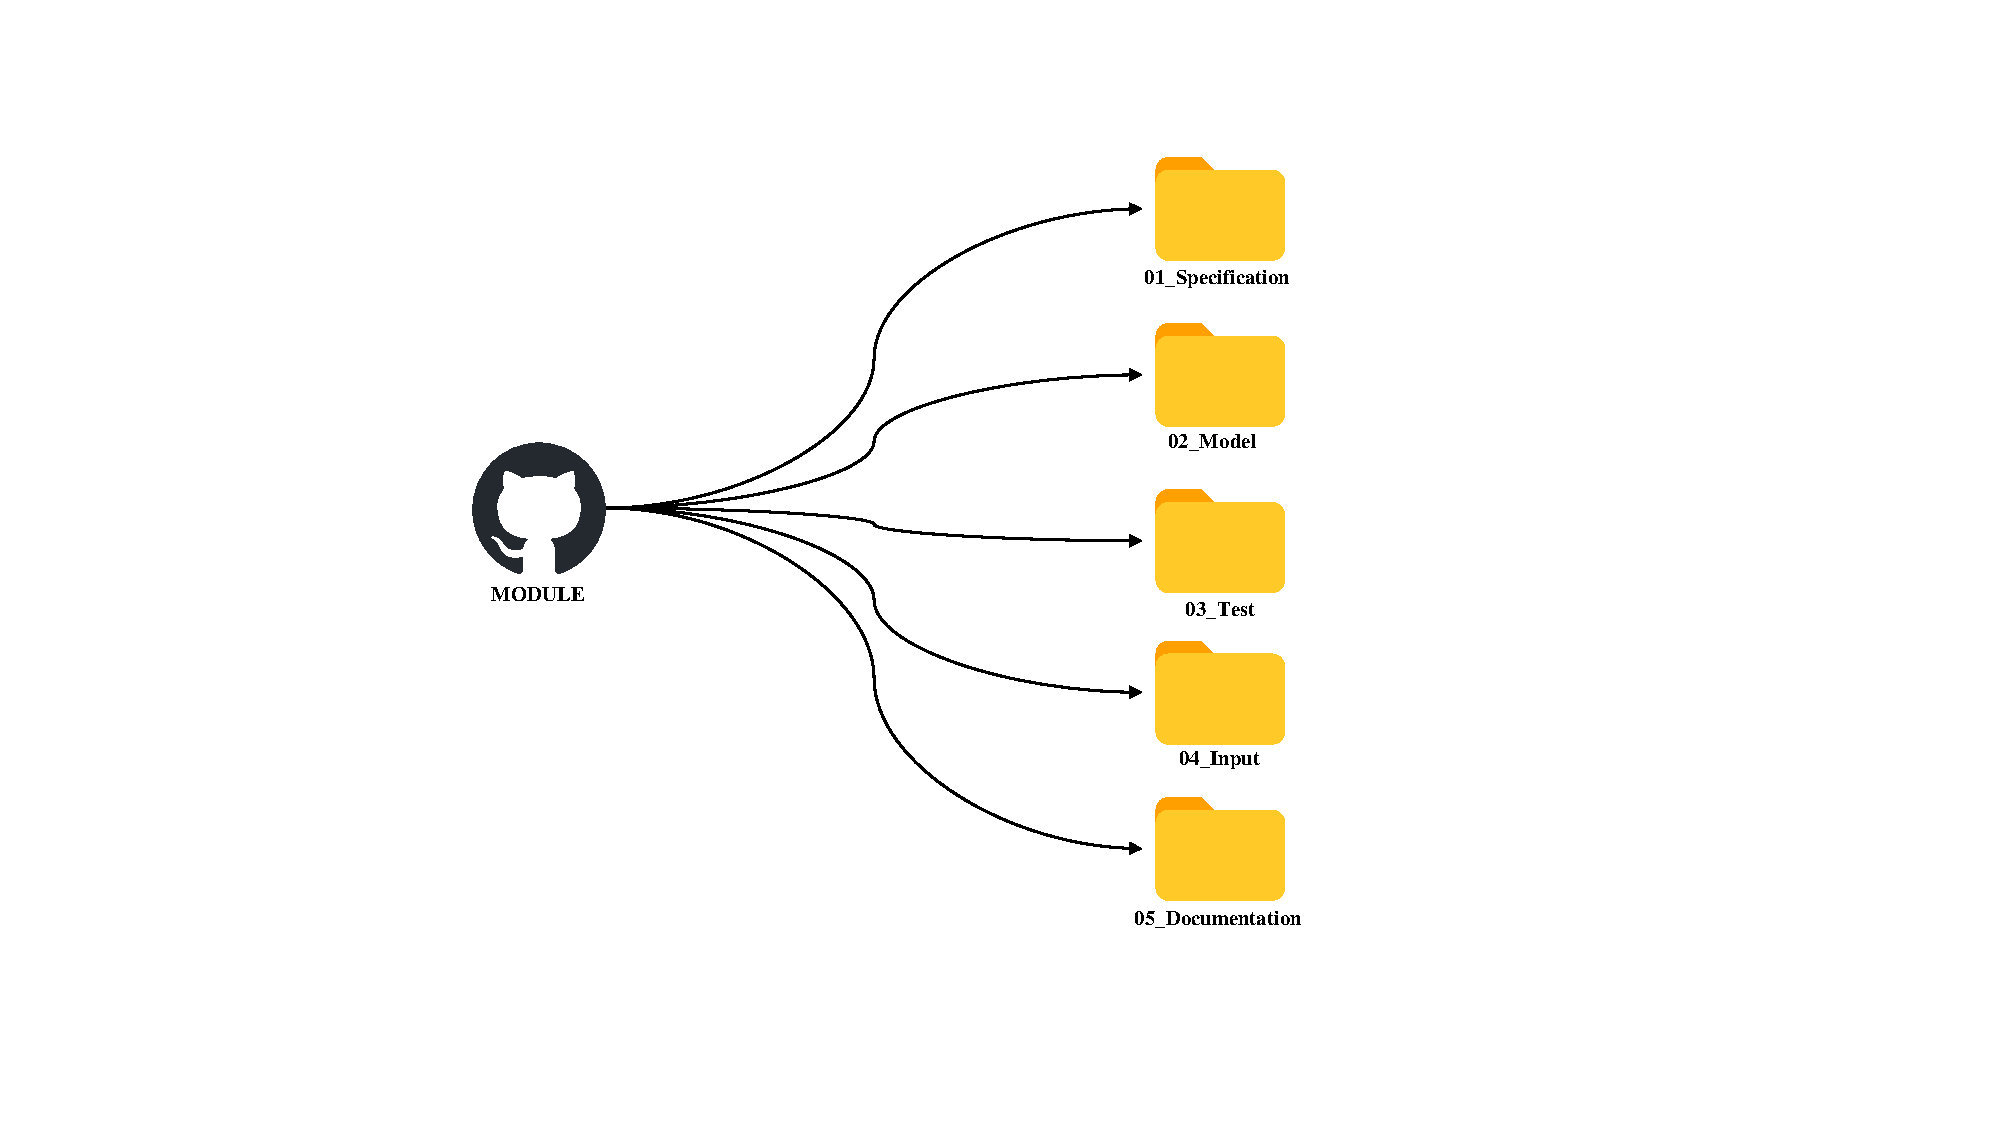
\includegraphics[width=1.2\textwidth]{Images/github_folder_structure.pdf}
    \caption{Example of a module's GitHub repository structure}
    \label{github_arrhenius}
\end{figure}

Figure \ref{github_arrhenius} shows us an example of how each module is maintained in our GitHub.
\begin{itemize}
    \item \verb|01_Specification| has all the requirements for the module to run.
    \item \verb|02_Model| contains all parts to run the model. This can also be used as a playground for the development of a model.
    \item \verb|03_Test| withholds all relevant documents regarding unit tests or integration test can be found here. This is one of the important part 
                        of the module.
    \item \verb|04_Input| carries all the initial parameters or functions to be defined at the start of a module.
    \item Documentation explaining functioning and usage of the module can be found under \verb|05_Documentation|.
\end{itemize}
%\begin{table}[!h]
%    \begin{tabular}{|>{\centering\arraybackslash}p{2cm}|>{\centering\arraybackslash}p{12cm}|}
%        \hline
%        Name of the module & \multirow{2}{*}{\centering Use Case}\\
%        \hline
%        Pv Calculator & Simulation of FET losses as input for the FET's temperature estimation as base for a first reliability prognosis\\
%    \end{tabular}
%\end{table}
\subsection{Workflows}
Our department develop automatized workflows for power electronics products considering functional loads to reliability indications. Workflows are a sequence
of modules designed for a fast calculation performance characteristic like temperature or reliability indication. To develop a workflow, Optislang is used.


Every architectural workflow has a GitHub repository that is maintained in a similar way to how modules are being maintained.

\begin{figure}[!h]
    \centering
    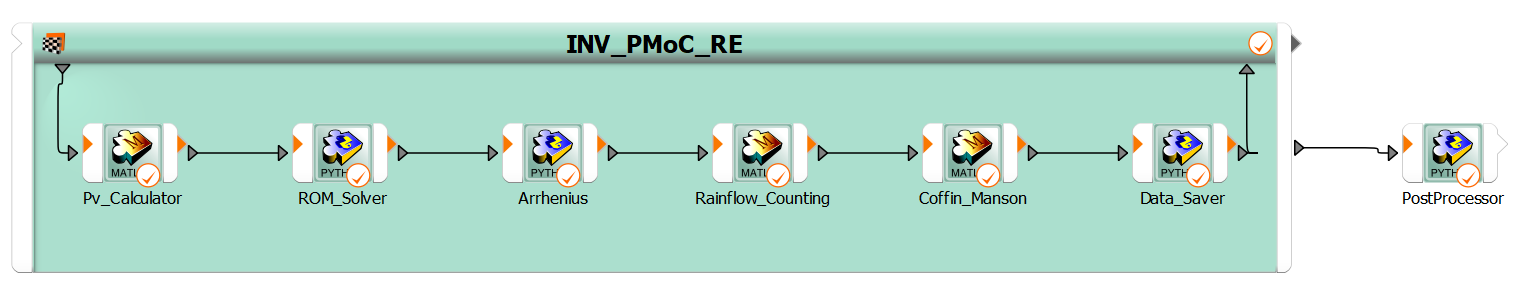
\includegraphics[width=\textwidth]{Images/workflow_example.png}
    \caption{Example of a workflow in Optislang}
    \label{workflow_example}
\end{figure}

%%%%%%%%%%%%%%%%%   SECTION : CURRENT PROBLEM   %%%%%%%%%%%%%%%%%%%%%%%%%%%%%%
\section{Current Problem} \label{current problem}
lorem ipsum dolor sit amet, consectetur adipiscing elit. Donec auctor, nunc nec lorem ipsum dolor sit amet, consectetur adipiscing elit. Donec auctor, nunc
nec lorem ipsum dolor sit amet, consectetur adipiscing elit. Donec auctor, nunc nec lorem ipsum dolor sit amet, consectetur adipiscing elit. Donec auctor, nunc
nec lorem ipsum dolor sit amet, consectetur adipiscing elit. Donec auctor, nunc nec lorem ipsum dolor sit amet, consectetur adipiscing elit. Donec auctor, nunc
nec lorem ipsum dolor sit amet, consectetur adipiscing elit. Donec auctor, nunc nec lorem ipsum dolor sit amet, consectetur adipiscing elit. Donec auctor, nunc
nec lorem ipsum dolor sit amet, consectetur adipiscing elit. Donec auctor, nunc nec lorem ipsum dolor sit amet, consectetur adipiscing elit. Donec auctor, nunc
lorem ipsum dolor sit amet, consectetur adipiscing elit. Donec auctor, nunc nec lorem ipsum dolor sit amet, consectetur adipiscing elit. Donec auctor, nunc
nec lorem ipsum dolor sit amet, consectetur adipiscing elit. Donec auctor, nunc nec lorem ipsum dolor sit amet, consectetur adipiscing elit. Donec auctor, nunc

 %#! Explain why it is time consuming to test the module, labour intensive, increase of errors with complexity of the module/workflow
 %#! Explain the lack of standardization of module, difficulty in maintaining the modules effectively